\documentclass[
a4paper,                        % paper size
11pt,                           % font size
twoside,                        % two sided
footsepline,                    % add a line to separate the footer
headsepline,                    % add a line to separate the header
headexclude,                    % header does not belong to the text
footexclude,                    % footer does not belong to the text
pagesize,                       % set the pagesize in a DVI document
bibtotocnumbered,               % add the bibliography to the TOC
idxtotoc                        % add the index to the TOC
%openright,                      % start a new chapter on the right page
%,DIV12
%,draft
]{scrreprt}

\usepackage{nameref}            % nameref, varioref, hyperref must be
                                % used in this order (see hyperref
                                % README)!
\usepackage[draft]{varioref}    % defines \vref
\usepackage{hyperref}           % automatically creates links when
                                % using pdflatex, defines \url
\usepackage{ifpdf}              % defines \ifpdf
\usepackage{graphicx}           % handles graphics
\usepackage{makeidx}            % creates the index
\usepackage{fancybox}

%%%%%%%%%%%%%%%%%%%%%%%%%%%%%%%%%%%%%%%%%%%%%%%%%%
%%%%%%%%%%%%%%%%%%%%%%%%%%%%%%%%%%%%%%%%%%%%%%%%%%
%%%%%%%%% New Commands and Environments %%%%%%%%%%
%%%%%%%%%%%%%%%%%%%%%%%%%%%%%%%%%%%%%%%%%%%%%%%%%%
%%%%%%%%%%%%%%%%%%%%%%%%%%%%%%%%%%%%%%%%%%%%%%%%%%
\newcommand{\es}{\textsf{ESPResSo}}
\newcommand{\ie}{\textit{i.e.\/}}
\newcommand{\eg}{\textit{e.g.\/}}
\newcommand{\etal}{\textit{et al.\/}}

\newcommand{\variant}[2]{(#1) \texttt{#2}\\}
%\newcommand{\lit}[1]{\texttt{#1}}
\newcommand{\var}[1]{\textrm{\textit{#1}}}
\newenvironment{syntax}{%
  \begin{Sbox}
    \begin{minipage}{0.9\linewidth}
    }{%
    \end{minipage}
  \end{Sbox}
  \begin{center}
    \fbox{\TheSbox}
  \end{center}
}

%%%%%%%%%%%%%%%%%%%%%%%%%%%%%%%%%%%%%%%%%%%%%%%%%%
%%%%%%%%%%%%%%%%%%%%%%%%%%%%%%%%%%%%%%%%%%%%%%%%%%
%%%%%%%%%%%%%%%% Other Settings %%%%%%%%%%%%%%%%%%
%%%%%%%%%%%%%%%%%%%%%%%%%%%%%%%%%%%%%%%%%%%%%%%%%%
%%%%%%%%%%%%%%%%%%%%%%%%%%%%%%%%%%%%%%%%%%%%%%%%%%
\pagestyle{headings}
\makeindex

%%%%%%%%%%%%%%%%%%%%%%%%%%%%%%%%%%%%%%%%%%%%%%%%%%
%%%%%%%%%%%%%%%%%%%%%%%%%%%%%%%%%%%%%%%%%%%%%%%%%%
%%%%%%%%%%%%%%%%% Main Document %%%%%%%%%%%%%%%%%%
%%%%%%%%%%%%%%%%%%%%%%%%%%%%%%%%%%%%%%%%%%%%%%%%%%
%%%%%%%%%%%%%%%%%%%%%%%%%%%%%%%%%%%%%%%%%%%%%%%%%%
\begin{document}
\titlehead{
  \begin{center}
    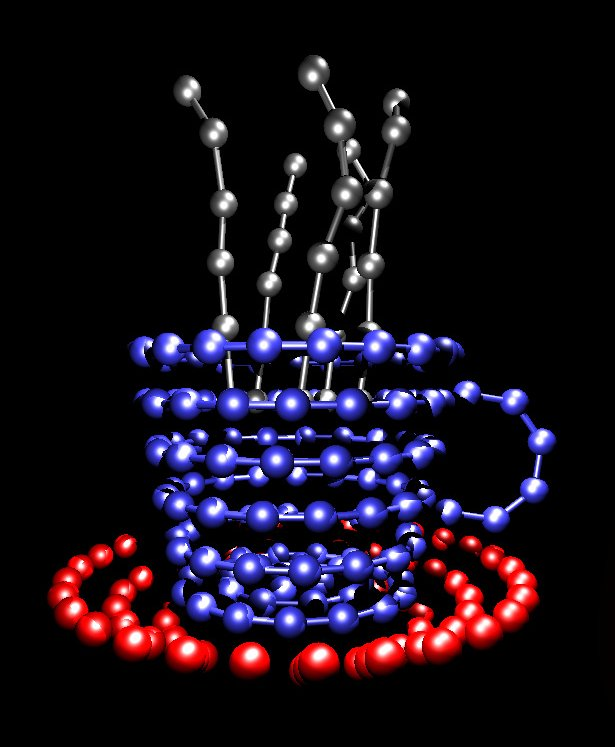
\includegraphics[width=5cm]{logo.jpg}
  \end{center}
}
%\subject{Dissertation}
\title{\es{} User's Guide}
%\author{Dipl.-Inform. Olaf~Lenz}
%\date{\today}
\maketitle

\tableofcontents

\chapter{Introduction}
\label{chap:intro}

(new)

\begin{itemize}
\item \es{} is a generic soft matter simulation packages
\item for molecular dynamics simulations in soft matter research
\item focussed on coarse-grained models
\item employs modern algorithms (Lattice-Boltzmann, DPD, P3M, \ldots)
\item written in C for maximal portability
\item Tcl-controlled
\item parallelized
\end{itemize}

\section{Guiding principles}
\label{sec:ideas}

(from paper: 2.1 Goals and principles)

\es
\begin{itemize}
\item does \emph{not} do the physics for you!
\item requires you to understand what you do (can not be used as a
  black box)
\item gives you maximal freedom (flexibility)
\item is extensible
\item integrates system setup, simulation and analysis, as this can't
  be strictly separated in soft matter simulations
\item has no predefined units
\item sets as few defaults as possible
\end{itemize}

\section{Algorithms contained in \es}

The following algorithms are implemented in \es{}:

\begin{itemize}
\item ensembles: NVE, NVT, NpT
\item charged systems:
  \begin{itemize}
  \item P3M for fully periodic systems
  \item ELC and MMM-family of algorithms for charged systems with
    non-periodic boundary conditions
  \item Maggs algorithm 
  \end{itemize}
\item Hydrodynamics:
  \begin{itemize}
  \item DPD (as a thermostat)
  \item Lattice-Boltzmann
  \end{itemize}
\end{itemize}

\section{Basic program structure}
\label{sec:structure}

(from paper: 2.2 Basic program structure)

\begin{itemize}
\item Control level: \texttt{Tcl}
\item ``Kernel'' written in \texttt{C}
\item This manual will focus on the control level
\end{itemize}

\section{On units}
\label{sec:units}

(new)

\begin{itemize}
\item Reduced units
\item comparison to ``real units''
\item three examples on different length scales
  \begin{itemize}
  \item some atomistic model?
  \item coarse-grained model (\eg lipid bilayer)
  \item billards?
  \end{itemize}
\end{itemize}

% Copyright (C) 2010,2011,2012,2013 The ESPResSo project
% Copyright (C) 2002,2003,2004,2005,2006,2007,2008,2009,2010 
%   Max-Planck-Institute for Polymer Research, Theory Group
%  
% This file is part of ESPResSo.
%   
% ESPResSo is free software: you can redistribute it and/or modify it
% under the terms of the GNU General Public License as published by the
% Free Software Foundation, either version 3 of the License, or (at your
% option) any later version.
%  
% ESPResSo is distributed in the hope that it will be useful, but
% WITHOUT ANY WARRANTY; without even the implied warranty of
% MERCHANTABILITY or FITNESS FOR A PARTICULAR PURPOSE.  See the GNU
% General Public License for more details.
%  
% You should have received a copy of the GNU General Public License
% along with this program.  If not, see <http://www.gnu.org/licenses/>.
%
\chapter{Getting, compiling and running \es}
\label{chap:install}
\index{Installation|textbf}

This chapter will describe how to get, compile and run the \es
software.  

\es releases are available as source code packages from the \es home
page\footnote{\url{http://espressomd.org}}.  This is where new users
should get the code.  The code within release packages is tested and
known to run on a number of platforms.  Alternatively, people that
want to use the newest features of \es or that want to start
contributing to the software can instead obtain the current
development code via the version control system software
\textsf{git}\footnote{\url{http://git.org}} from \es's project page at
the Savannah GNU server
\footnote{\url{https://savannah.nongnu.org/projects/espressomd/}}.
This code might be not as well tested and documented as the release
code; it is recommended to use this code only if you have already
gained some experience in using \es.

Unlike most other software, no binary distributions of \es are
available, and the software is usually not installed globally for all
users.  Instead, users of \es should compile the software themselves.
\index{features} The reason for this is that it is possible to
activate and deactivate various features before compiling the code.
Some of these features are not compatible with each other, and some of
the features have a profound impact on the performance of the code.
Therefore it is not possible to build a single binary that can satisfy
all needs.  A user should always activate only those features that are
actually needed.  This means, however, that learning how to compile
\es is a necessary evil.  The build system of \es uses the GNU
autotools, which are developed since more than 20 years and allow to
compile software easily on a wide range of platforms.

\section{Running \texttt{configure}}
\label{sec:configure}
\index{configure}

\todo[inline]{Description of basic options: \keyword{CPPFLAGS},
  \keyword{CFLAGS}, \keyword{LDFLAGS}}

The first step of building \es is to run the shell script
\codebox{configure} which is to be found in the top level source
directory.  The script collects all the information required by the
compilation process.  It will determine how to use and where to find
the compiler, as well as the different libraries and tools required by
the compilation process, and it will test what compiler flags are to
be used.  The script will find out about most of these things
automatically.  If something is missing, it will complain and give
hints how to solve the problem.  The generic syntax of calling the
\codebox{configure} script is:
\begin{code}
configure [\var{options} ...] [\var{variable}=\var{value} ...]
\end{code}

If you are using the development source code from the \textsf{git}
repository, before you can call \codebox{configure}, it is necessary
to have the GNU autotools (\textsf{autoconf} and \textsf{automake})
installed. Then you can call the script \codebox{bootstrap.sh} from
the top level source directory, which will generate the
\codebox{configure} script.

\subsection{Source and build directories}
\label{ssec:builddir}
\index{build directory} \index{source directory}

Usually, when a program is compiled, the resulting binary files are
put into the same directory as the sources of the program.  In \es's
build system, the \emph{source directory} that contains all the source
files is completely separated from the \emph{build directory}, where
the files created by the build process are put.  The location of the
build directory is the current working directory at the time when
\codebox{configure} is called.  In this way, you can build several
variants of \es, each variant having different activated features, and
for as many platforms as you want.  All further commands concerning
compiling and running \es have to be called from the build directory.

\paragraph{Example}
When the source directory is \codebox{\$srcdir} (\ie the files where
unpacked to this directory), then the build directory can be set to
\codebox{\$builddir} by calling the \codebox{configure}-script from
there:
\begin{code}
cd $builddir
$srcdir/configure
make
Espresso
\end{code}

\subsection{Options}
\label{ssec:configureoptions}

\index{configure options} The behaviour of \codebox{configure} can be
controlled by the means of command line options.  In the following
only those command line options that are specific to \es will be
explained.  For a complete list of options and explanations thereof,
call
\begin{code}
configure --help
\end{code}

\begin{description}
\item[\texttt{--with-myconfig=MYCONFIG\_HEADER}] This option sets the
  name of the local configuration header (see \vref{sec:myconfig}). It
  defaults to ``\texttt{myconfig.h}''.
\item[\texttt{--with-mpi=\alt{\lit{yes} \asep \lit{no} \asep
      \lit{guess}}}/ \texttt{--without-mpi}] By default,
  \codebox{configure} will automatically determine whether an MPI
  compiler is available.  If it is, it will use it.  If you specify
  \codebox{--without-mpi} or \codebox{--with-mpi=no}, then MPI will
  not be used, even if it is available.
\item[\texttt{--with-efence} / \texttt{--without-efence}] Whether or
  not to use the ``electric fence'' memory debugging library.
  \footnote{\url{http://freshmeat.net/projects/efence/}} Efence is not
  used by default.
\item[\texttt{--with-tcl=TCL}] By default, \texttt{configure} will
  automatically determine which version of Tcl is used.  If the wrong
  version is chosen automatically, you can specify the name of the
  library with this option, \eg \texttt{tcl8.4}.
\item[\texttt{--with-tk=TK} / \texttt{--without-tk}] By default, the
  GUI toolkit Tk is not used by \es. This option can be used to
  activate Tk and to specify which Tk version to use, \eg{}
  \texttt{tk8.4}. If you only specify \texttt{--with-tk} and do not
  give a version number, \texttt{configure} will try to automatically
  deduce the right version.
\item[\texttt{--with-fftw} / \texttt{--without-fftw}] This can
  be used to specify whether the FFTW library is to be used, and which
  version.  By default, version 3 will be used if it is found,
  otherwise version 2 is used.  Note that quite a number of central
  features of \es require FFTW.
\item[\texttt{--with-cuda=path} / \texttt{--without-cuda}] This switch
  enables CUDA support. \texttt{path} should be the path to the CUDA
  directory, which can be omitted if it is the NVIDIA default path,
  \ie \texttt{/usr/local/cuda}. The variable \texttt{NVCCFLAGS} can
  be used to define compiler flags for the NVIDIA CUDA-compiler
  \texttt{nvcc}. For example, \texttt{NVCCFLAGS = "{}-gencode
    arch=compute_20,code=sm_20"{}} will compile code only for Fermi
  cards.  Default is to compile for compute models 1.1 and 2.0,
  i.e. everything with a G90 chip or newer.  Note that we require at
  least compute model 1.1.
\end{description}

\section{\texttt{make}: Compiling,  testing and installing \es}
\label{sec:make}

The command \texttt{make} is mainly used to compile the \es source
code, but it can do a number of other things. The generic syntax of
the \texttt{make} command is:
\begin{code}
make [\var{options}] [\var{target}...] [\var{variable}=\var{value}]
\end{code}
When no target is given, the target \texttt{all} is used. The
following targets are available:
\begin{description}
\item[\texttt{all}] Compiles the complete \es source code. The
  variable \lit{myconf} can be used to specify the name of the
  configuration header to be used.
\item[\texttt{check}] Runs the testsuite. By default, all available
  tests will be run on 1, 2, 3, 4, 6, or 8 processors. Which tests are
  run can be controlled by means of the variable \texttt{tests}, which
  processor numbers are to be used can be controlled via the variable
  \texttt{processors}. Note that depending on your MPI installation,
  MPI jobs can only be run in the queueing system, so that \es{} will
  not run from the command line. In that case, you may not be able to
  run the testsuite, or you have to directly submit the testsuite script
  \verb!testsuite/test.sh! to the queueing system.\\
  \textbf{Example:} \verb!make check tests="madelung.tcl" processors="1 2"!\\
  will run the test \texttt{madlung.tcl} on one and two processors.
\item[\texttt{clean}] Deletes all files that were created during the
  compilation.
\item[\texttt{mostlyclean}] Deletes most files that were created
  during the compilation. Will keep for example the built doxygen
  documentation and the \es{} binary.
\item[\texttt{dist}] Creates a \texttt{.tar.gz}-file of the \es{}
  sources.  This will include all source files as they currently are
  in the source directory, \ie{} it will include local changes.  This
  is useful to give your version of \es{} to other people.
  The variable \texttt{extra} can be used to specify additional
  files and directories that are to be included in the archive
  file. \\
  \textbf{Example:} \verb!make dist extra="myconfig.h internal"!\\
  will create the archive file and include the file
  \texttt{myconfig.h} and the directory \texttt{internal} with all
  files and subdirectories.
\item[\texttt{install}] Install \es. The variables \texttt{prefix} and
  \texttt{exec-prefix} can be used to specify the installation
  directories, otherwise the defaults defined by the
  \texttt{configure} script are used. \texttt{prefix} sets the prefix
  where all \es files are to be installed, \texttt{exec-prefix} sets
  the prefix where the executable files are to be installed and is
  required only when there is an architecture-specific directory.\\
  \textbf{Example:} \verb!make install prefix=/usr/local!\\
  will install all files below \texttt{/usr/local}.
\item[\texttt{uninstall}] Uninstalls \es, \ie removes all files that
  were installed during \texttt{make install}. The variables are
  identical to the variables of the \texttt{install}-target.
\item[\texttt{ug\ \ }] Creates the User guide in the \texttt{doc/ug}
  subdirectory (only when using the development sources).
\item[\texttt{dg\ \ }] Creates the Developers' guide in the
  \texttt{doc/dg} subdirectory (only when using the development
  sources).
\item[\texttt{doxygen\ \ }] Creates the Doxygen code documentation in the
  \texttt{doc/doxygen} subdirectory.
\item[\texttt{tutorials\ \ }] Creates the \es tutorials in the
  \texttt{doc/tutorials} subdirectory.
\item[\texttt{doc\ }] Creates all documentation in the \texttt{doc}
  subdirectory (only when using the development sources).
\end{description}

A number of options are available when calling \texttt{make}.  The
most interesting option is probably \texttt{-j \textit{num\_jobs}},
which can be used for parallel compilation on computers that have more
than one CPU or core.  \textit{num\_jobs} specifies the maximal number
of jobs that will be run.  Setting \textit{num\_jobs} to the number of
available processors speeds up the compilation process significantly.

\section{Running \es}
\label{sec:run}

When \es is found in your path, it can be run via
\begin{code}
Espresso [\var{tcl\_script} [\var{args}]]
\end{code}

\index{interactive mode} When \es{} is called without any arguments,
it is started in the interactive mode, where new commands can be
entered on the command line. When the name of a \textit{tcl\_script}
is given, the script is executed. \textit{N\_processors} is the number
of processors that are to be used. Any further arguments are passed to
the script. Note that depending on your MPI installation, MPI jobs can
only be run in the queueing system, so that \es will not run from
the command line.


\section{\texttt{myconfig.h}: Activating and deactivating features}
\label{sec:myconfig}

\index{features} \index{myconfig.h} \index{configuration header} \es
has a large number of features that can be compiled into the binary.
However, it is not recommended to actually compile in all possible
features, as this will slow down \es significantly.  Instead, compile
in only the features that are actually required.  A strong gain in
speed can be achieved, by disabling all non-bonded interactions except
for a single one, e.g. \feature{LENNARD_JONES}.  For the developers,
it is also possible to turn on or off a number of debugging messages.
The features and debug messages can be controlled via a configuration
header file that contains C-preprocessor declarations. Appendix
\vref{chap:features} lists and describes all available features.  When
no configuration header is provided by the user, a default header,
found in src/myconfig-default.h, will be used that turns on the
default features.  The file \texttt{myconfig-sample.h} in the source
directory contains a list of all possible features that can be copied
into your own configuration file.

When you distinguish between the build and the source directory, the
configuration header can be put in either of these. Note, however,
that when a configuration header is found in both directories, the one
in the build directory will be used.

By default, the configuration header is called \texttt{myconfig.h}.
The name of the configuration header can be changed either when the
\texttt{configure}-script is called with the option
\mbox{\texttt{--with-myconfig}} (see section \vref{sec:configure}), or
when \texttt{make} is called with the setting
\mbox{\texttt{myconfig=}\textit{myconfig\_header}} (see section
\vref{sec:make}).

The configuration header can be used to compile different binary
versions of \es with a different set of features from the same source
directory.  Suppose that you have a source directory \texttt{\$srcdir}
and two build directories \texttt{\$builddir1} and
\texttt{\$builddir2} that contain different configuration headers:

\begin{itemize}
\item \texttt{\$builddir1/myconfig.h}:
\begin{code}
#define ELECTROSTATICS
#define LENNARD-JONES
\end{code}

\item \texttt{\$builddir2/myconfig.h}:
\begin{code}
#define LJCOS
\end{code}
\end{itemize}

\noindent Then you can simply compile two different versions of \es via
\begin{code}
cd $builddir1
$srcdir/configure
make

cd $builddir2
$srcdir/configure
make
\end{code}


%%% Local Variables: 
%%% mode: latex
%%% TeX-master: "ug"
%%% End: 


\chapter{Tutorial}
\label{chap:tutorial}

(from \verb!erice_tutorial! or appendix A from paper)

\begin{itemize}
\item \es: script interpreter
\item interactive use (sample session)
\item script execution
\item example script
\item Reference to \verb!tutorial.tcl! (?)
\end{itemize}

# Feature definitions
#
# The definitions are used for
# * generation of src/config-features.hpp, which checks the sanity of
#   the various features and their combinations
# * generation of myconfig-sample.hpp
#
# Copying and distribution of this file, with or without modification,
# are permitted in any medium without royalty provided the copyright
# notice and this notice are preserved.  This file is offered as-is,
# without any warranty.
#
# Lines commented with '/* ... */' or '//' are copied to myconfig-sample.hpp
# Lines commented with '#' are ignored

/* Generic features */
EXTERNAL_FORCES
MASS
EXCLUSIONS
BOND_CONSTRAINT
LANGEVIN_PER_PARTICLE
COLLISION_DETECTION
METADYNAMICS
NPT
SWIMMER_REACTIONS
ENGINE                          implies ROTATION, EXTERNAL_FORCES
PARTICLE_ANISOTROPY             implies ROTATION

/* Rotation */
ROTATION
ROTATIONAL_INERTIA              implies ROTATION

/* Electrostatics */
ELECTROSTATICS
P3M                             equals ELECTROSTATICS and FFTW
MMM1D_GPU                       requires CUDA and ELECTROSTATICS
_P3M_GPU_FLOAT                  requires CUDA and ELECTROSTATICS

/* Magnetostatics */
DIPOLES                         implies ROTATION
DP3M                            equals DIPOLES and FFTW
DIPOLAR_DIRECT_SUM              requires CUDA
DIPOLAR_DIRECT_SUM              equals DIPOLES and ROTATION and CUDA

DIPOLAR_BARNES_HUT              requires CUDA
DIPOLAR_BARNES_HUT              equals DIPOLES and ROTATION and CUDA

/* Virtual sites features */
VIRTUAL_SITES                   
VIRTUAL_SITES_RELATIVE          implies VIRTUAL_SITES
VIRTUAL_SITES_RELATIVE          implies ROTATION

VIRTUAL_SITES_INERTIALESS_TRACERS
VIRTUAL_SITES_INERTIALESS_TRACERS implies VIRTUAL_SITES

/* DPD features */
DPD

/* Lattice-Boltzmann features */
LB_BOUNDARIES
LB_BOUNDARIES_GPU               requires CUDA
LB_ELECTROHYDRODYNAMICS
ELECTROKINETICS                 implies EXTERNAL_FORCES, ELECTROSTATICS
ELECTROKINETICS                 requires CUDA
EK_BOUNDARIES                   implies ELECTROKINETICS, LB_BOUNDARIES_GPU, EXTERNAL_FORCES, ELECTROSTATICS
EK_BOUNDARIES                   requires CUDA
EK_DEBUG                        requires ELECTROKINETICS
EK_DOUBLE_PREC                  requires ELECTROKINETICS

/* Interaction features */
TABULATED
LENNARD_JONES
WCA
LENNARD_JONES_GENERIC           implies LENNARD_JONES
LJCOS
LJCOS2
LJGEN_SOFTCORE                  implies LENNARD_JONES_GENERIC
GAY_BERNE                       depends EXPERIMENTAL_FEATURES
SMOOTH_STEP
HERTZIAN
GAUSSIAN
BMHTF_NACL
MORSE
BUCKINGHAM
SOFT_SPHERE
HAT
UMBRELLA                           requires EXPERIMENTAL_FEATURES
GAY_BERNE                       implies ROTATION
GAY_BERNE
OVERLAPPED
THOLE                           requires ELECTROSTATICS

/* Fluid-Structure Interactions (object in fluid) */
OIF_LOCAL_FORCES
OIF_GLOBAL_FORCES
AFFINITY requires EXPERIMENTAL_FEATURES
MEMBRANE_COLLISION requires EXPERIMENTAL_FEATURES

/* Immersed-Boundary Bayreuth version */
SCAFACOS_DIPOLES                requires SCAFACOS
SCAFACOS_DIPOLES                implies DIPOLES
SCAFACOS                        requires ELECTROSTATICS

EXPERIMENTAL_FEATURES

/* Strange features. Use only if you know what you are doing! */
/* turn off certain nonbonded interactions within molecules */
NO_INTRA_NB                     notest

/* Debugging */
ADDITIONAL_CHECKS

COMM_DEBUG
EVENT_DEBUG
HALO_DEBUG
P3M_DEBUG
THERMO_DEBUG
VIRTUAL_SITES_DEBUG
CUDA_DEBUG
H5MD_DEBUG


# External switches
# Switches that are set by configure or gcc, not to be set manually
CUDA external
FFTW external
H5MD external
SCAFACOS external
GSL external


\chapter{\es{} command reference}
\label{chap:ref}

(most from paper and from related pages)

\begin{itemize}
\item Will contain description of all Tcl-commands
\item Reference to appendix \vref{chap:quickref}
\item basic identifiers:
  \begin{itemize}
  \item particle type
  \item bonded interaction type
  \item molecule id
  \end{itemize}
\end{itemize}


\section{\texttt{inter}: Setting up interactions}
\label{sec:inter}
\begin{syntax}
  \variant{1}
  {inter 
    \var{part\_type\_id1} 
    \var{part\_type\_id2}
    \var{inter\_type} 
    [ \var{parameters}\ldots ]
  }
  \variant{2}
  {inter 
    \var{bond\_type\_id} \var{bond\_type} [
    \var{parameters}\ldots ]
  }
  \variant{3}
  {inter}
\end{syntax}
    % \section{Creating particles}
% \label{sec:part}
% \texttt{part}

% \section{Interactions}
% \label{sec:inter}
% \texttt{inter}

% \section{Analysis}
% \label{sec:analysis}

\chapter{Under the hood}
\label{chap:underhood}

(new)

\begin{itemize}
\item Implementation issues that are interesting for the user
\item Main loop in pseudo code (for comparison)
\item from doxygen: ``Cell systems'' 
\end{itemize}


\chapter{Getting involved}
\label{chap:devel}

\begin{itemize}
\item What to do when you want to become involved
\item How to submit a bug report
\end{itemize}


\appendix
\chapter{\es{} quick reference}
\label{chap:quickref}

\begin{itemize}
\item Short reference table of all commands
\item Complete syntax of \es{} commands
\item Features required for different commands
\end{itemize}

\chapter{The MMM family of algorithms}
\label{chap:mmm}

\chapter{Maggs algorithm}
\label{chap:maggs}

\printindex

\end{document}


%%% Local Variables: 
%%% mode: latex
%%% TeX-master: t
%%% End: 
